\chapter{Introduction}
\section{Historical overview}
Clusters of galaxies are the largest and most recent gravitationally-relaxed
structures in the universe. They typically contain hundreds to thousands of
galaxies with a total mass of about $10^{14} - 10^{15}$ solar masses
($\unit{M_{\odot}}$), spread over a region whose size is roughly 10 million
light-years ($\unit{Mly}$). Galaxy clusters themselves form even greater
structures called superclusters, which are gravitationally-attracted, but not
relaxed, collections of ten to one hundred clusters and groups of galaxies. The
Milky
Way itself belongs to the ``Local Group'' , which is an aggregation of
about 40 galaxies, with the Andromeda Galaxy and the Milky Way as the largest
members of
the group. The Local Group belongs to the ``Virgo Supercluster'', with the
Virgo cluster at the center. The Virgo cluster is the nearest cluster of
galaxies to our own galaxy at a distance of 60 Mly; another famous cluster of
galaxies is the Coma cluster, which is called a very regular cluster,
because it is nearly spherically symmetric (see figure \ref{fig:comavis}).
\begin{figure}[tp]
\centering
\includegraphics[width=0.7\linewidth]{chapter1/Comacluster_nasajpl.eps}
\caption{A Sloan Digital Sky Survey/Spitzer Space Telescope image of the Coma
Cluster in ultraviolet and visible light. From \citet{Jenkins2007}.}
\label{fig:comavis}
\end{figure}

The tendency of galaxies to form clusters in the sky has long been noticed (for
example \citet{Messier1784} had identified already 16 galaxies, which - as we
now know - belong to the Virgo cluster, and he noted that they form a
group), but
the first to study them in detail was \citet{Wolf1906}. A great step forward in
the systematic study of the properties of clusters was the work of
\citet{Abell1958}, who compiled the first extensive, statistically complete
catalog of so-called rich clusters of galaxies\footnote{The richness of a galaxy
is a measure that is basically proportional to the number of bright galaxies in
a cluster. It was first strictly defined by Abell for his catalog.}. This
catalog and its successors (e.g. \citet{Abell1989}) are the foundation for much
of our modern understanding of clusters.   

The cited catalogs of clusters are based on optical identification techniques.
However in the early 1970s extended x-ray emission from clusters of galaxies
was observed by \citet{Gursky1971, Kellogg1972}, which had been already
correctly attributed to thermal
bremsstrahlung several years earlier by \citet{Felten1966}. This interpretation
requires
the space between galaxies in clusters to be filled with a very hot 
($\approx \unit[10^8]{K}$) low density ($\approx \unit[10^3]{atoms/m^3}$) gas.
Remarkably, the total mass in this intracluster medium (ICM) is comparable to
the total mass of all galaxies in the cluster. Nevertheless this discovery did
not solve the so called missing mass problem in clusters, which was first
formulated by \citet{Zwicky1933,Zwicky1937}. \citet{Zwicky1933} was the first
to measure the velocity dispersion of galaxies in the Coma cluster, finding
$\sigma_{galaxy}=\unit[700]{km\ s^{-1}}$, and he correctly concluded from this
fact and his estimate of the Coma's cluster overall radius, that the cluster
mass, which he computed using the virial theorem, must be far greater than the
observed luminous mass - the first evidence for dark matter in the universe. In
his remarkable paper of 1937, Zwicky also proposed gravitational lensing as an
alternative technique for measuring the masses of background galaxies. This
technique finally became practicable after six more decades \citep{Tyson1990},
and is now a standard technique for measuring cluster mass
\citep{Bartelmann2003}.

Measuring the masses of clusters is not only important for the search of dark
matter. Some of the most powerful constraints on current cosmological models
come from observations of how the cluster mass function $n(M)$, which gives the
number density of clusters with a mass greater than $M$ in comoving volume
element, evolves with time \citep{Voit2005}. The reason why the evolution of the
cluster mass function is so highly sensitive to cosmology is simply because the
matter density of the universe controls the rate at which structure grows. 
The cluster mass function can be measured using optical surveys.
However it is easier to use X-ray surveys, because in the X-ray band, instead of
a collection of galaxies, each cluster appears only as a single source (see
figure \ref{fig:comaxray}), 
\begin{figure}[tp]
\centering
\includegraphics[width=0.62\linewidth]{chapter1/0150_xray.eps}
\caption{Chandra X-ray image of the central region of the Coma Cluster. From
\citet{Vikhlinin2002}.}
\label{fig:comaxray}
\end{figure}
which makes it observationally easier to define consistently
cluster properties like the radius. Independently from Supernova IA and cosmic
microwave background (CMB) measurements, these and other cluster-related
surveys can now restrict several important parameters of the cosmological
concordance model (see figure \ref{fig:omegas}). 
\begin{figure}[tp]
\centering
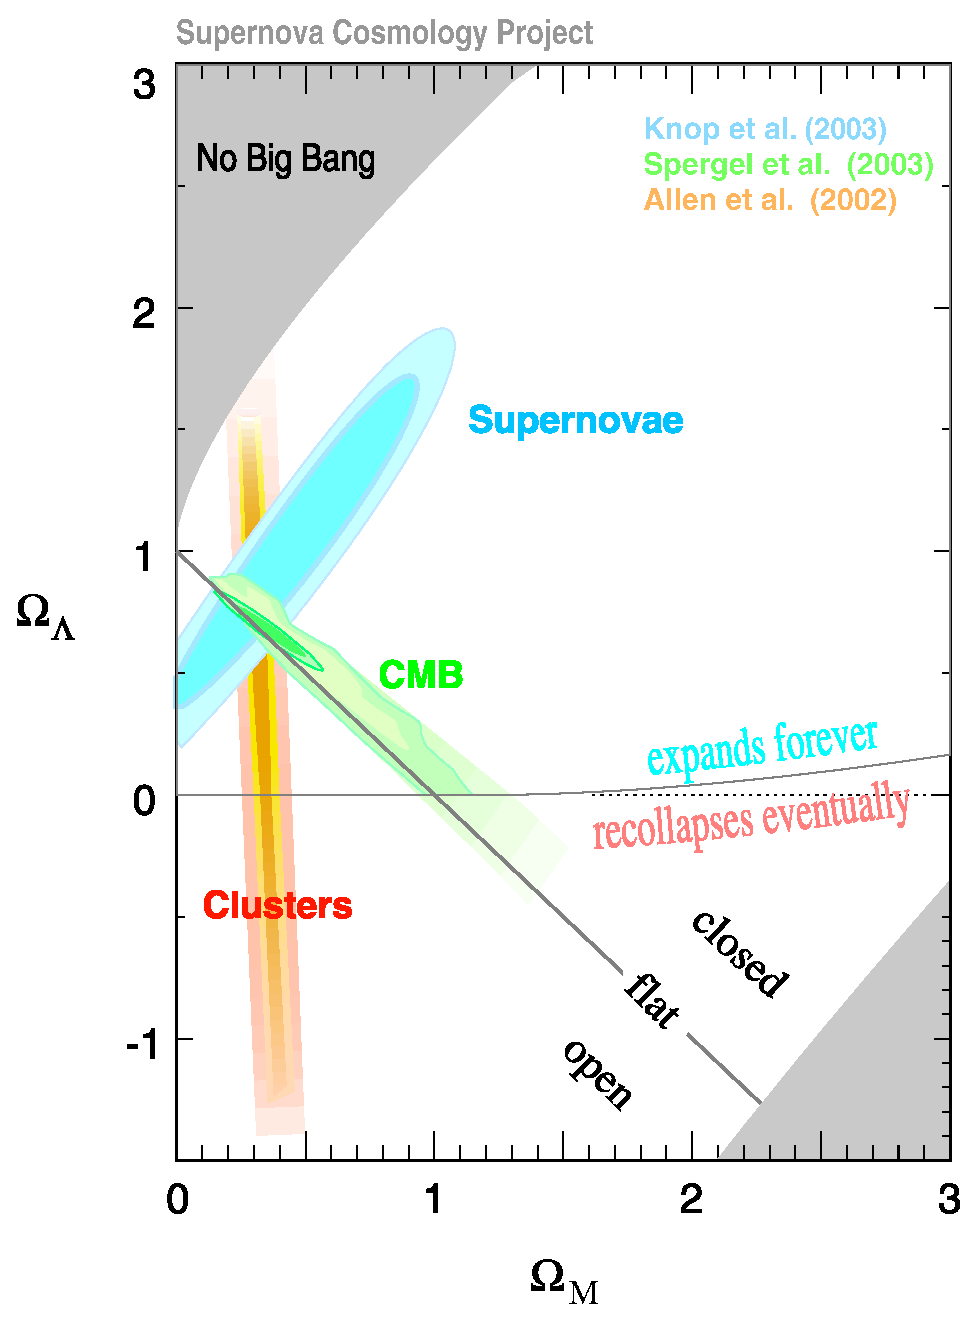
\includegraphics[width=0.45\linewidth]{chapter1/SCP2003SNeCMBClust.eps}
\caption{Plot of 68\% and 90\% confidence regions for $\Omega_M$
and $\Omega_{\Lambda}$ for Supernova IA, CMB and cluster data. From
\citet{Knop2003}.
}
\label{fig:omegas}
\end{figure}

Most of these cluster surveys make use of several
relations like the mass-temper\-ature or luminosity-temperature relation, which
are only based on observational findings. If gravity alone would determine
the thermodynamical properties of the clusters, we would expect clusters to be
self-similar, meaning clusters of different size would be scaled versions of
each other, leading to a specific simple form of these relations
\citep{Kaiser1986}.
However astronomers have known for more than a decade that the intracluster
medium cannot be self-similar, because the luminosity-temperature
relation of clusters does not agree with self-similar scaling \citep{Voit2005}.
So only by breaking the self-similar scaling of clusters can the
observed relations be explained. But it is theoretically
still uncertain, which mechanism(s) is (are) responsible for that similarity
breaking. Many mechanisms have been proposed including preheating, radiative
cooling, feedback from supernovae, feedback from active galactic nuclei
\citep{Voit2005}, shocks, magnetic fields, cosmic rays and turbulence 
\citep{Dolag2008}. It therefore remains a challenge for the theory of cluster
physics to find the responsible mechanisms and explain the relations mentioned
above.

\section{Aim of this work}
One of the proposed mechanisms that break gravitationally self-similar scaling
properties of clusters is turbulence. Turbulence is also believed to
play an important role in explaining the magnetic field strengths of galaxy
clusters and the higher than expected temperature of cluster cores (the 
``cooling flow problem''). However numerical simulations of the
influence of turbulence in an astrophysical context in general and especially
for clusters have been restricted to measuring passively statistical
quantities
like velocity dispersion from simulation data (e.g. \citet{Dolag2005}). 
The active role of small scale velocity fluctuations on the large scale flow
could not be treated at all. There are two main reasons for this:
\begin{enumerate}
\item Basically turbulence is a physical phenomenon that is far from
being understood. The sole currently  existing theory is only
applicable to isotropic, incompressible turbulence. No accepted theoretical
framework for
describing turbulent flows in astrophysical environment including compressible,
selfgravitating, high Mach number flows exists. 
\item Models describing the effective influence of turbulence in fluid dynamic
simulations are restricted to a specific length scale. They are not suitable to
treat the vast range of different length scales (from cosmological scales
$\approx \unit[10^{24}]{m}$
down to the thickness of a shock front ($\approx \unit[10^{11}]{m}$,
\citet{Medvedev2006}) we need to address
when simulating astrophysical environments.
\end{enumerate}
Therefore it is aim of this work to develop, implement, and apply a new
numerical scheme for modeling turbulent, multiphase astrophysical flows such as
galaxy cluster cores and star forming regions. The method combines the
capabilities of adaptive mesh refinement (AMR) and large-eddy simulations (LES)
to capture localized features and to represent unresolved turbulence,
respectively; it will be referred to as Fluid mEchanics with
Adaptively Refined Large-Eddy SimulationS or FEARLESS. 

To start explaining the idea behind this ansatz, we first give a brief overview
of the theory of turbulence in chapter \ref{turbulence}. In chapter \ref{filter}
we introduce a filter formalism, which is necessary for modeling compressible
turbulence according to the ideas of LES. In chapter \ref{FE} we use this
formalism to derive the filtered equations of fluid dynamics, which are the
basis for the introduction of our turbulence or subgrid scale (SGS) model
(adapted from work by \citet{Schmidt2006}) in chapter \ref{LES}.
In this chapter we also analyse in some detail the
influence of the turbulence model on the equation of fluid dynamics. In chapter
\ref{amrles} we explain the specific problem of combining LES and AMR in
some detail and propose a new method to circumvent this problem. In chapter
\ref{numtest} we comment on several modifications and numerical issues that
had to be taken into account when implementing our method into the cosmological
fluid code Enzo. We also present the results of several driven turbulence test
simulations, showing the consistency of our treatment of turbulence. Chapter
\ref{clustertheo} summarizes some important facts about cluster physics and we
also give a brief introduction to turbulence in cluster simulations.
In chapter \ref{clustersim} we describe several issues with our turbulence model
when treating turbulence in cluster simulations on cosmological scales. We
explain our setup and then describe the main results of a first study of
turbulence in galaxy cluster simulations using our FEARLESS approach. Finally in
chapter \ref{summ} we
summarize our findings and draw conclusions about the influence of turbulence
in the context of cluster simulations. 

